\documentclass[acmlarge]{acmart}

\AtBeginDocument{%
  \providecommand\BibTeX{{%
    Bib\TeX}}}

%% ============================================================
%% RIGHTS / METADATA
%% For a course submission (not an official ACM publication) you can
%% leave these as-is or simplify. They do not affect grading.
%% If you want to remove the "ACM Reference Format" / copyright strip,
%% you may add \settopmatter{printacmref=false} below.
%% ============================================================
\settopmatter{printacmref=false}      % hide ACM reference block (course doc, not a real ACM paper)
\setcopyright{none}                   % no copyright line
\renewcommand\footnotetextcopyrightpermission[1]{} % kill the copyright footnote

\begin{document}

%% ============================================================
%% TITLE
%% ============================================================
\title{WayBack: A Context-Aware Recommender System for Re-Finding Personal Information in Tourism}

%% ============================================================
%% AUTHORS  (use full names exactly as on TUM transcripts)
%% ============================================================
\author{Haichen Duan}
\email{haichen.duan@tum.de}
\affiliation{%
  \institution{Technical University of Munich}
  \city{Munich}
  \country{Germany}}

\author{Swayamsidh Mohanty}
\email{swayamsidh.mohanty@tum.de}
\affiliation{%
  \institution{Technical University of Munich}
  \city{Munich}
  \country{Germany}}

\renewcommand{\shortauthors}{Duan and Mohanty}

%% ============================================================
%% ABSTRACT   (write LAST, ~150-200 words)
%% One paragraph: problem (re-finding in tourism), what you built
%% (3 methods from Sappelli adapted to tourism, deployed app),
%% how you evaluated (four layers: offline, diary, user study, tests),
%% headline result (method ordering reproduces the paper on real data).
%% ============================================================
\begin{abstract}
% DRAFT (shared section) --- review jointly before submission.
Travellers routinely save places to maps, screenshots, and notes, yet
rarely return to them: the information is not lost but effectively
unfindable. This is a \emph{re-finding} problem, distinct from the
discovery task most tourism recommenders address. We adapt the
context-aware re-finding framework of Sappelli, Verberne, and Kraaij
(2017), originally developed for office documents, to personal tourism
information. We implement their three methods---a content-based
recommender (CBR), a just-in-time information-retrieval ranker (JITIR),
and a contextual interactive-activation network (CIA)---together with a
random baseline, and expose them through WayBack, a deployed responsive
web application that re-surfaces previously saved places by current
location and time. We evaluate on four layers: a reproducible offline
experiment over simulated Munich tourist sessions, a one-week diary study
on real accumulated data, a mixed-methods user study, and an automated
test suite. Offline, the paper's separation of roles reproduces: CBR maximises
context precision, and CIA is strongest at placing the next action first
and at catalogue coverage; a week of real use qualitatively confirms the
same separation, and users find the moment-aware JITIR ranking most
useful. No
single method dominates every criterion, confirming that
re-finding is best served by complementary rankers rather than a single
model.
\end{abstract}

%% ============================================================
%% CCS + KEYWORDS  (generate real CCS codes at https://dl.acm.org/ccs
%% e.g. Information systems -> Recommender systems. Fill before submit.)
%% ============================================================
\begin{CCSXML}
<ccs2012>
   <concept>
       <concept_id>10002951.10003317.10003347.10003350</concept_id>
       <concept_desc>Information systems~Recommender systems</concept_desc>
       <concept_significance>500</concept_significance>
   </concept>
   <concept>
       <concept_id>10003120.10003121.10011748</concept_id>
       <concept_desc>Human-centered computing~Empirical studies in HCI</concept_desc>
       <concept_significance>300</concept_significance>
   </concept>
</ccs2012>
\end{CCSXML}

\ccsdesc[500]{Information systems~Recommender systems}
\ccsdesc[300]{Human-centered computing~Empirical studies in HCI}

\keywords{recommender systems, information re-finding, context-aware recommendation, tourism, user study}

\maketitle

%% ============================================================
%% CONTENTS  (book-style front matter: title + abstract, then a
%% clean contents page of its own, then the body starts fresh)
%% ============================================================
\clearpage
\begingroup
  \hypersetup{linkcolor=black}% TOC entries in plain black, book-like
  \setcounter{tocdepth}{2}%   sections and subsections, no deeper
  \tableofcontents
\endgroup
\clearpage

%% ============================================================
%% 1. INTRODUCTION & MOTIVATION   [owner: shared / Joan lead]
%% ============================================================
\section{Introduction and Motivation}
\label{sec:intro}

Travellers accumulate saved places. A restaurant is bookmarked on a map, a
museum survives as a screenshot, a bar recommended by a friend ends up in a
note. Much of this information is never used again, not because it lost its
value but because it does not resurface at the moment it would be useful.
Returning to it is a \emph{re-finding} problem: the target is known and
already stored, and success means recovering it in the right situation
rather than discovering something new.

Tourism recommender systems overwhelmingly address the opposite task.
They suggest places the user has not seen, and they are evaluated on how
well those suggestions match inferred preferences~\cite{borras2014tourism}.
The complementary task of returning a traveller to their own saved places
has received little attention, even though re-retrieval accounts for a
substantial share of information behaviour in
general~\cite{teevan2007reretrieval}. Context makes the task tractable.
Whether a saved place is worth resurfacing depends on where the user is,
what time it is, and what the weather permits, and these signals are
available to a mobile application at the moment of use.

Sappelli, Verberne, and Kraaij~\cite{sappelli2017} studied exactly this
problem for office documents. They proposed three context-aware
recommendation methods from different traditions, together with four
evaluation criteria that capture distinct notions of a good suggestion,
and found that no single method wins on all four. This report transfers
their framework to tourism and asks whether the framework, and its central
finding, survive the move. Our contributions are:

\begin{enumerate}
  \item an adaptation of the three methods (JITIR, CBR, and CIA) and a
        random baseline to tourism items and tourism context, with each
        design decision traceable to the original paper
        (Section~\ref{sec:methods});
  \item WayBack, a publicly deployed web application in which every
        recommendation is drawn from the user's own saved pool, so the
        re-finding constraint is enforced by construction
        (Sections~\ref{sec:system-design} and~\ref{sec:frontend});
  \item an evaluation on four layers: a reproducible multi-seed offline
        experiment, a week-long diary study on real accumulated data
        rather than seed data, a mixed-methods user study, and an
        automated test suite. Across these layers the paper's central
        finding reproduces: no single method dominates every criterion,
        and the methods are complementary
        (Section~\ref{sec:offline} onwards).
\end{enumerate}

The remainder of the report is organised as follows. Section~\ref{sec:background}
reviews re-finding and the Sappelli framework. Section~\ref{sec:methodology}
describes the methods as implemented for tourism and the interaction design
built around them. Section~\ref{sec:implementation} covers the
implementation of the frontend and the backend.
Section~\ref{sec:evaluation} presents the four evaluation layers, and
Section~\ref{sec:conclusion} concludes with limitations and future work.


%% ============================================================
%% 2. RELATED WORK / BACKGROUND   [owner: shared]
%% ============================================================
\section{Background and Related Work}
\label{sec:background}

\subsection{Re-Finding versus Discovery}
Most recommender systems perform \emph{discovery}: they predict items a
user has never seen and might like. \emph{Re-finding} is the complementary
task of returning a user to information they have already encountered and
stored. Teevan et al.~\cite{teevan2007reretrieval} showed that a large
fraction of web activity is re-retrieval of previously seen results rather
than discovery of new ones, and that the two tasks have different success
criteria: re-finding is judged by whether the \emph{known} target is
recovered, not by novelty. In tourism this distinction is sharp. A
traveller accumulates saved places across maps, bookmarks, tickets, and
notes, but the act of \emph{returning} to the right saved place at the
right moment is unsupported by the discovery-oriented tools that dominate
the domain~\cite{borras2014tourism}. WayBack targets this gap: it never
suggests anything outside the saved pool---every recommendation is an item
already stored in the app---and re-surfaces that pool ranked by present
context.

\subsection{The Sappelli Re-Finding Framework}
Our work is a direct adaptation of Sappelli, Verberne, and
Kraaij~\cite{sappelli2017}, who studied context-aware recommendation for
re-finding personal \emph{office} documents. Their study contributes two
things we reuse. First, a set of three recommendation methods rooted in
different traditions: a just-in-time information-retrieval agent (JITIR), a
content-based recommender (CBR), and a contextual interactive-activation
network (CIA). Second, a four-part evaluation rubric that measures
qualitatively different notions of a ``good'' suggestion:

\begin{itemize}
  \item \textbf{Context relevance} --- does the suggestion fit the user's
        current situation (in our case, the active place category)?
  \item \textbf{Document relevance} --- how much does the suggested item's
        content overlap the user's current task text?
  \item \textbf{Action prediction} --- did the system rank the item the
        user accesses next near the top?
  \item \textbf{Diversity} --- across successive moments, does the system
        vary its suggestions and cover the catalogue, or repeat itself?
\end{itemize}

The central empirical finding of the paper---that no single method wins on
all four criteria, so the methods are complementary---is the hypothesis we
re-test on tourism data (Section~\ref{sec:offline}).

\subsection{Lineage of the Three Methods}
Each method descends from an established line of work. The \textbf{CBR}
method is a classical content-based recommender built on TF--IDF
term weighting and cosine similarity~\cite{salton1988tfidf}: it represents
each saved place as a bag-of-words vector and ranks by similarity to a
query built from the current context. \textbf{JITIR} follows the
just-in-time information-retrieval paradigm of Rhodes and
Maes~\cite{rhodes2000jitir}, in which a background agent continuously turns
the user's current context into a query and retrieves matching documents;
we realise the retrieval step with BM25~\cite{robertson2009bm25}, the
modern probabilistic ranking function, in place of the paper's Indri
default. \textbf{CIA} is a spreading-activation network in the interactive-activation
tradition of McClelland and Rumelhart~\cite{mcclelland1981iac}: context
signals activate a middle layer of context-information nodes, which spread
activation to saved items and back. WayBack sits within the broader field
of context-aware recommendation~\cite{adomavicius2011context} and tourism
recommendation~\cite{borras2014tourism}, but is distinguished by its
re-finding objective and its faithful reproduction of the Sappelli method
suite.

%% ============================================================
%% 3. METHODOLOGY   [owner: Sway lead on methods, Joan on design]
%% ============================================================
\section{Methodology}
\label{sec:methodology}

\subsection{The Three Methods and Baseline}
\label{sec:methods}

All four rankers implement a common interface: given the saved pool and a
\emph{context} object, they return the top-$k$ items, each with a score
and a short explanation. The context is assembled per request from the
client's latitude and longitude, an optional active category, free-text
query, and weather tag, with the current time taken from the server's UTC
clock; the weather tag is consumed only by the explanation layer below,
so the rankers work from text, category, location, and time. When the
client sends no text, the backend substitutes a time-of-day query (e.g.\
``lunch food market restaurant'' between 11:00 and 14:00) from the same
clock, so the methods never disagree near an hour boundary. Each saved
item contributes a text document concatenating its title, description,
tags, and category; Table~\ref{tab:method-map} maps each method to its
paper section and in-app labels.

\begin{table}[t]
  \caption{Mapping of the three methods to their source in
  Sappelli et al.~\cite{sappelli2017} and to the user-facing tab labels.}
  \label{tab:method-map}
  \begin{tabular}{llll}
    \toprule
    Method & Paper \S & In-app tab & Compare label \\
    \midrule
    JITIR & 5.1 & For this moment & Relevant \\
    CBR   & 5.2 & Based on history & Similar \\
    CIA   & 5.3 & Near you & Contextual \\
    \bottomrule
  \end{tabular}
\end{table}

\subsubsection{CBR --- Content-Based Recommender.}
CBR (``Based on history'') ranks in two steps. It first
\emph{pre-filters} the pool to items whose category equals the active
context category, reproducing the paper's contextual pre-filtering; with no
active category the full pool passes through. It then scores the remaining
items by TF--IDF cosine similarity to a query document built from the
context text, using raw term counts weighted by a smoothed logarithmic
inverse document frequency~\cite{salton1988tfidf}; the corpus over which
frequencies are computed is the pre-filtered pool plus the query document
itself, so term weights adapt to the active category.
When the context carries no query text, CBR falls back to a neutral
constant score so that the category pre-filter alone determines the
result. Because the pre-filter guarantees every surviving item matches the
active category, CBR is by construction strong on context relevance and
weak on cross-category diversity---a trade-off the evaluation confirms.

\subsubsection{JITIR --- Just-In-Time Information Retrieval.}
JITIR (``For this moment'') treats the whole context as a search query and
ranks the \emph{entire} pool with no pre-filter, following Rhodes and
Maes~\cite{rhodes2000jitir}. The query concatenates the context text and
the active category; retrieval uses BM25~\cite{robertson2009bm25} with the
standard parameters $k_1=1.5$ and $b=0.75$ and a smoothed probabilistic
inverse document frequency. Items with a non-zero score are returned in
descending order. Because JITIR scores across the whole pool rather than
inside one category, it trades some context precision for the ability to
surface a strongly matching item from an adjacent category---exactly the
``for this moment'' behaviour its label promises.

\subsubsection{CIA --- Contextual Interactive Activation.}
CIA (``Near you'') is the most involved method: a three-layer
spreading-activation network in the interactive-activation
tradition~\cite{mcclelland1981iac}, rebuilt per request so it stays in
sync with the pool. The layers are \emph{event} (the current context),
\emph{context-information} nodes, and \emph{items}. Context-information
nodes are extracted from each saved item and come in four kinds: topic
nodes (one per text token), a category node, a location node obtained by
snapping the coordinates to a $\sim$0.005$^\circ$ grid cell so that nearby
places share a node, and a time-of-day node when the item has an event
time. Each item is linked to the context nodes it generates.

Activation follows Grossberg's bounded update rule. With inhibition set to
zero (the paper uses excitation only), one update of an activation $a$
under excitatory input $e$ is
\begin{equation}
  \Delta a = (a_{\max}-a)\,e - \delta\,(a-a_{\mathrm{rest}}),
  \qquad
  a \leftarrow \mathrm{clip}\big(a+\Delta a,\,a_{\min},\,a_{\max}\big),
\end{equation}
with bounds $a_{\min}=-0.1$, $a_{\max}=1.0$, rest $a_{\mathrm{rest}}=-0.1$,
and decay $\delta=0.1$. Connection weights follow the paper's Table~3
normalisation: a context node excites an item in inverse proportion to its
number of out-links, and an item excites a context node in inverse
proportion to the size of its own context set.
The current context seeds the context layer: query tokens share one unit
of activation (tokens absent from the item-derived vocabulary are
discarded), and the active category, location cell, and time bucket each
contribute a full unit. The network runs ten iterations, each a forward
pass in which items accumulate excitation from their context nodes and a
backward, pseudo-relevance-feedback pass in which context nodes accumulate
excitation from items plus a re-injection of the original event
activation, so the seed signal persists rather than decaying away. The
final activation is the item's score; like JITIR, CIA returns only items
with strictly positive activation, so an item with no matching context
links is dropped rather than ranked at its resting level. Because activation reaches an item through several context paths
at once---topic, category, location, and time---CIA most rewards items
coherent with the whole situation, which is why the paper and our results
find it strongest at next-action prediction and catalogue coverage.

\subsubsection{Random Baseline.}
The random baseline returns a uniform sample of $k$ items with a constant
score. It lives only in the offline harness---the serving API exposes the
three context-aware methods---and marks the floor any method must clear;
Section~\ref{sec:offline} shows it also exposes which metrics are
sensitive to pool size rather than to ranking quality. Each instance owns
a seeded generator so that multi-seed runs do not share state.

\subsubsection{Explanation Layer.}
Independently of the ranker, the backend attaches a human-readable reason
to every recommendation. A rule function inspects the real item data
(distance, save age, view count, indoor category, current weather) and
emits a compact reason code such as \texttt{matches\_weather\_indoor} or
\texttt{nearby\_frequent\_view}; the frontend maps each code to display
text, and the method's own scoring detail is carried alongside for
transparency. This keeps the \emph{why} of a recommendation grounded in
observable facts rather than in the opaque score.

\subsection{System Design and Interaction}
\label{sec:system-design}

Section~\ref{sec:methods} describes what the rankers compute; this section
describes the interaction design built around them. A single constraint
applies to every surface of the application: it never displays a place the
user has not saved, so the saved pool is the entire catalogue. This
constraint carries a design consequence. A discovery system can compensate
for a weak ranking by introducing new items, whereas a re-finding system
cannot, and the interface must therefore make the provenance of each item
visible and the ranking itself credible.

\paragraph{Save.}
Re-finding presupposes a prior save, and saves typically happen in
transit, so the flow is designed to impose minimal friction. A place enters the pool in one of two ways: through
a search field, which queries an OpenStreetMap geocoder and fills the save
form from the result, or through a pin drop on the map, which always works
and does not depend on geocoder coverage (Section~\ref{sec:diary}). The
save form carries a free-text note alongside the name, following
Sappelli et al.~\cite{sappelli2017}, who treat a personal annotation as a
contextual cue that a name alone does not provide. The rankers consume this
cue directly, since the note text enters the item document that CBR, JITIR,
and CIA score against. The interface therefore makes the note easy to add
at save time and, as the diary study showed to be necessary, editable after
saving, because the relevance of a place often becomes clear only later.

\paragraph{Re-find.}
The map is the home surface. Saved places appear as category markers, and
above them sits a row of three tabs which are the three rankers of
Section~\ref{sec:methods}. The app opens on ``For this moment'' (JITIR),
the moment-aware ranking, rather than on the highest-precision one, a
default the offline and user-study layers both support
(Sections~\ref{sec:offline} and~\ref{sec:userstudy}). Switching tabs
re-ranks the same pool, so the user sees the methods disagree over items
they already own. Selecting a place opens a detail panel with the reason
for its rank, its distance and time signals, and an entry point to
navigation.

\paragraph{Why.}
Every recommendation carries a reason, produced by the rule-based
explanation layer of Section~\ref{sec:methods} and rendered as a short
sentence with a strength bar. The strength bar presents a coarse level rather than a numeric score,
because method scores are not comparable across rankers: a cosine
similarity, a BM25 value, and a network activation lie on different scales,
and displaying the raw numbers side by side would invite a comparison the
numbers cannot support. Each reason is grounded in facts the user can
verify independently, such as distance, time of day, weather, and how long
ago the place was saved.

\paragraph{Compare.}
A separate compare view puts the three rankings side by side on the same
pool, with each column normalised within itself and the raw score moved to
a tooltip. The compare view is the only surface where the paper's method terminology
appears in the product, and the naming is layered accordingly. In the map
and the detail panel the tabs read ``For this moment'', ``Based on
history'', and ``Near you'', which describe the result the user receives.
In the compare view the columns read ``Similar'', ``Relevant'', and
``Contextual'', with the corresponding Sappelli section reference as a
small tertiary label (Table~\ref{tab:method-map}). The two layers serve
different audiences: end users receive descriptive labels, while
technically interested readers can trace each column to its method. The
user study confirms that the labels are legible and also indicates the
limit of surface labelling, since participants read ``Near you'' as a
distance sort although it is driven by context activation
(Section~\ref{sec:userstudy}).

\paragraph{Plan.}
The day plan assembles saved places into five time slots, from a morning
cafe through to an evening restaurant or bar. The plan is itself a
re-finding surface, in that it arranges the saved pool rather than
generating new suggestions. A slot with no matching place is omitted rather
than filled, so a sparse pool yields a shorter plan rather than an
incorrect one.

\paragraph{The proactive channel.}
One recommendation is pushed rather than pulled: a banner over the map
surfaces a single place that fits the present context. Because unsolicited
recommendations risk becoming interruptions, the channel is bounded.
Dismissing the banner silences it for 45 minutes or until the user moves
more than 500 metres, on the assumption that a dismissal expresses
disinterest in the moment rather than in the specific item. Places outside
their opening hours are demoted rather than removed, and the detail panel
states the reason, because a re-finding system serves intents the user
already holds, including places saved for a future visit.

These decisions are carried by a visual system, Editorial Paper, whose
tokens, typography, and governance are described in
Section~\ref{sec:frontend}.


%% ============================================================
%% 4. IMPLEMENTATION   [owner: Joan frontend, Sway backend]
%% ============================================================
\section{Implementation}
\label{sec:implementation}

\subsection{Frontend and Design System}
\label{sec:frontend}

The client is a single-page React 19 application built with Vite and routed
with \texttt{react-router-dom}. The map surface uses \texttt{react-leaflet}
over Leaflet, and icons come from \texttt{lucide-react}. The codebase is
organised around two page components, the map page and the trip page that
hosts the day plan, together with a shared tab bar, and all chrome styling
is consolidated into a single global stylesheet. We use no CSS framework
and no component library; styling is hand-written CSS on top of a token
layer, which keeps every visual decision explicit in our own code rather
than inherited from a framework's defaults. This control matters because
the visual language carries part of the design argument described in
Section~\ref{sec:system-design}.

\begin{figure}[!t]
  \centering
  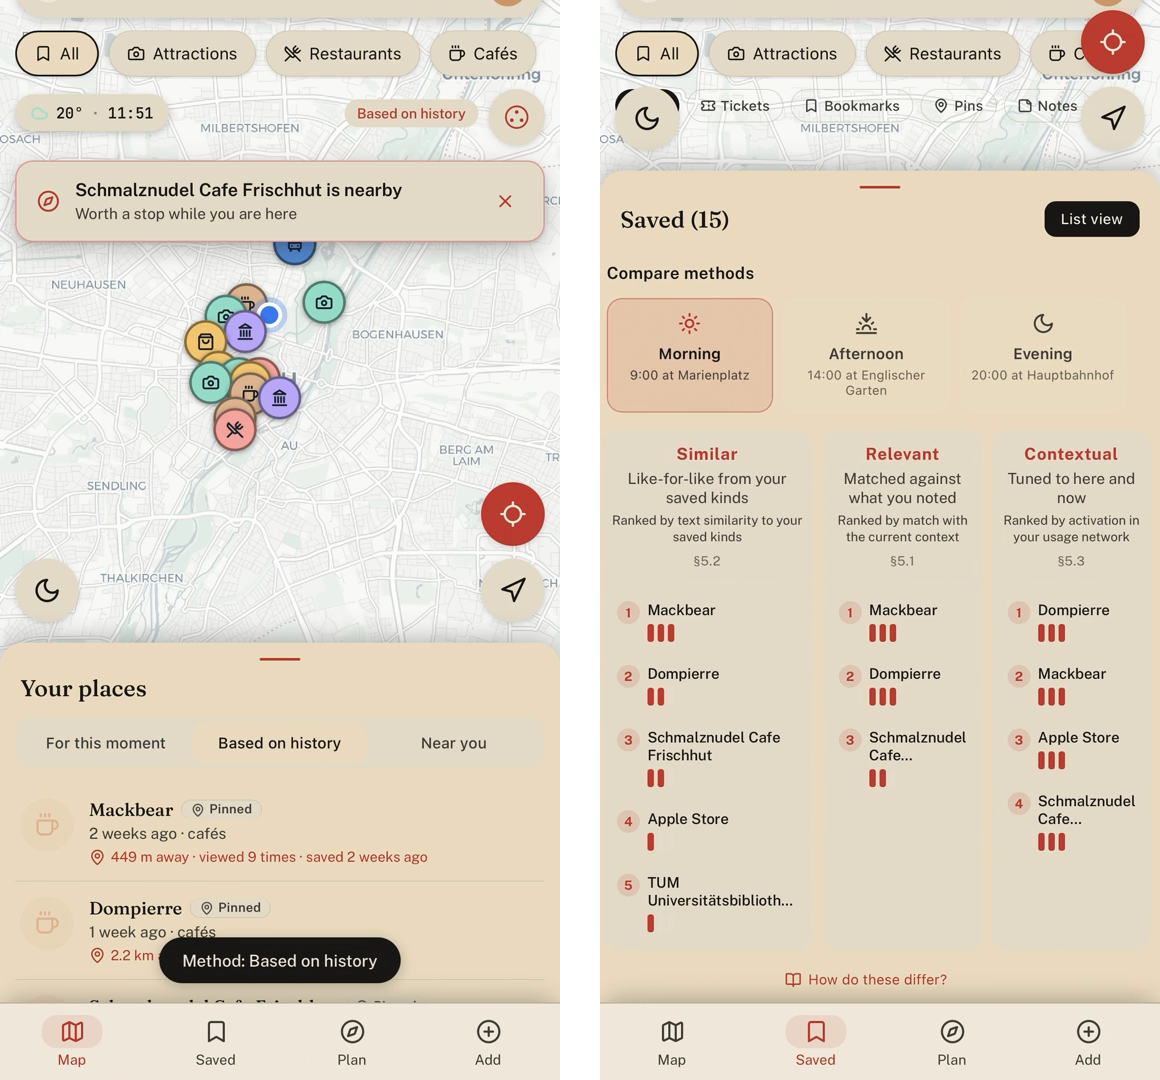
\includegraphics[width=0.58\linewidth]{ui_two_panel.png}
  \caption{Left: the map surface with the three method tabs and the
  recommendation sheet; saved places appear as desaturated category markers
  on Positron tiles. Right: the compare view, where the three rankings sit
  side by side under the labels Similar, Relevant, and Contextual, each
  column normalised within itself.}
  \Description{Two mobile screenshots of WayBack in light mode: the map
  view and the three-column compare view.}
  \label{fig:ui}
\end{figure}


The design system is called Editorial Paper. It is specified in a versioned
document, \texttt{docs/DESIGN.md}, which serves as the source of truth for
every visual and interaction decision in the frontend. The palette is a
cream paper family for surfaces (\texttt{--paper}, \texttt{--paper-soft},
\texttt{--paper-warm}), ink for text and structure (\texttt{--ink},
\texttt{--ink-soft}, \texttt{--rule}), and a single warm red accent
(\texttt{--pin}). The type stack pairs Fraunces for display, Public Sans
for body and interface copy, and JetBrains Mono for numerals such as
distances, times and scores, on a fixed scale from 12 to 48 pixels. The ten
category colours survive only as desaturated map-marker fills and are
banned from the chrome, so category distinction in the interface comes from
icon, label and typography rather than colour blocks. The map surface is integrated into the same palette, with CartoDB Positron
tiles in light mode. A warm dark counterpart, deep cocoa surfaces with
CARTO Dark Matter tiles, is toggled through a \texttt{data-theme} attribute
on the document root; the choice persists in local storage and is applied
before React mounts, so the first paint already uses the correct theme.

Two frontend features supply context signals the recommender consumes.
Place search uses Photon, a free OpenStreetMap geocoder, debounced at
300~ms and biased towards the user's position, with OSM tag pairs mapped
onto our ten categories and falling back to \emph{attraction} when a tag is
unrecognised. Geolocation is opt-in through \texttt{watchPosition}; until
the user grants permission, Munich Hauptbahnhof serves as the default frame
of reference and as the permanent fallback on denial.

Treating the design system as an artifact rather than a style guide
required enforcement. We wrote \texttt{design-check}, a static checker that
scans the frontend source and exits non-zero on any violation of the
anti-pattern bans that can be detected reliably: em dashes in user-facing
copy, the generic placeholder avatar, and the default drag handle. Bans
that cannot be distinguished from their sanctioned replacement by a static
marker are excluded from the checker rather than risking false
positives. The checker runs on
every push through GitHub Actions alongside the frontend unit tests
(Section~\ref{sec:tests}). \texttt{DESIGN.md} also carries a decision log,
which records reversals as well as decisions: the dark counterpart above
was removed and later re-introduced, and one anti-pattern ban was withdrawn
when the M2 walkthrough showed the banned element was doing useful
explanatory work. Recording reversals keeps the document an accurate account of the
system's history rather than an idealised one.



\subsection{Backend and Deployment}
\label{sec:backend}

The backend is a Flask service over an SQLAlchemy data model with two
domain tables. An \texttt{Item} stores a saved place---title, description,
item type, category, coordinates, address, optional event time, free-text
tags---plus behavioural fields: \texttt{created\_at}, which the
explanation layer turns into a months-since-saved signal, and
\texttt{last\_viewed\_at} with \texttt{view\_count}, the access-pattern
record maintained by the view endpoint below. The rankers themselves score
on text, category, location, and event-time context
(Section~\ref{sec:methods}); the access-pattern record feeds only the
explanation layer and is kept clean for a future access-based ranking
extension. A \texttt{Feedback} row records a useful / not-useful judgement
with the method and a context snapshot, so per-method success rates can be
aggregated for evaluation.

\paragraph{Request flow.}
A recommendation request is handled in four stages: the route validates
the query parameters (coordinates are required; \texttt{method} defaults
to CIA for bare API calls, though the app UI always sends one explicitly
and opens on the JITIR tab) and assembles the context object of
Section~\ref{sec:methods}; the selected ranker scores the pool; a scoring
stage augments each result with derived facts (haversine distance, months
since saved) that the explanation layer turns into a reason code; and the
item is serialised to the frontend's camelCase contract. The REST surface
covers reads, create, notes editing, and delete on saved items;
\texttt{GET /recommendations} with \texttt{method}, \texttt{top\_k}
(default five), and the optional context parameters of
Section~\ref{sec:methods}; and \texttt{POST /feedback} with an aggregate
\texttt{GET /feedback/stats} returning per-method success rates. The
contract's \texttt{userId} is accepted but not enforced: the prototype is
deliberately single-user for the study, and authentication is an
explicitly deferred item in the API contract.

\paragraph{Two data-integrity decisions driven by re-finding.}
Two endpoints keep the recorded behavioural signals honest. First,
recording a view is separated from reading:
\texttt{GET /saved-items/:id} is a pure read, while a deliberate open is
posted to \texttt{POST /items/:id/view}, debounced to ten
minutes---without the split, an incidental refresh or polling client
would inflate \texttt{view\_count} and corrupt the record behind the
``frequently viewed'' explanations. Second, the create endpoint
de-duplicates: a save whose name matches an existing item within fifty
metres returns HTTP~409 with the existing item, added after dogfooding
produced duplicate saves that polluted the pool, the rankings, and the
day plan (Section~\ref{sec:diary}).

\paragraph{Deployment and the persistence migration.}
The API is deployed on Render and the frontend on Vercel; allowed CORS
origins are configurable by environment variable. The seed is a
hand-curated pool of thirty Munich places spanning the ten place
categories; descriptions are baked into the seed once rather than
generated per request, so no live model call is made on the serving path.
The most consequential backend change was forced by real use: the service
initially ran on SQLite on Render's free tier, whose ephemeral disk reset
the pool to seed data on every deploy, and during the diary study this
destroyed a night's worth of real saves and---because re-finding is
evaluated on \emph{accumulated personal} data---invalidated that day's
evaluation. We migrated to a managed Neon Postgres instance and made the
seed script idempotent, seeding only an empty table, so the pool survives
deploys and cold starts. Smaller fixes from the same period: legacy
\texttt{postgres://} URLs are normalised, connections are pre-pinged
because Neon drops idle ones, and the feedback timestamp column was
widened to 64 bits after unix-millisecond values overflowed it; without
\texttt{DATABASE\_URL} the service falls back to local SQLite for
development and tests.

%% ============================================================
%% 5. EVALUATION AND RESULTS   [LONGEST SECTION]
%% This is the strongest section. Four subsections = your four layers.
%% ============================================================
\section{Evaluation and Results}
\label{sec:evaluation}
% One intro paragraph (shared): four layers, on REAL dogfooded data.

We evaluate WayBack on four complementary layers, each answering a
question the others cannot. An \emph{offline experiment}
(Section~\ref{sec:offline}) compares all four methods on the four paper
criteria under controlled, reproducible conditions. A one-week
\emph{diary study} (Section~\ref{sec:diary}) checks whether the same
behaviour holds on real, accumulated data rather than on the balanced seed
pool. A \emph{user study} (Section~\ref{sec:userstudy}) brings in people
who did not build the app. An automated \emph{test suite}
(Section~\ref{sec:tests}) guards the metric implementations and the
determinism the offline layer relies on. A recurring theme is that results
on the seed pool and results on real data can diverge, so we report both
and treat agreement across layers as the strongest evidence.

\subsection{Offline Evaluation}
\label{sec:offline}

\paragraph{Protocol.}
The offline experiment compares the four rankers on the six metrics that
operationalise the paper's four criteria (Table~\ref{tab:metric-map}). A
seeded, reproducible session simulator drives the methods: a session
visits eight of ten well-known Munich hotspots without revisits on a
fixed simulated date, each event carrying a noisy location, an advancing
clock (30--90 minutes between stops), the hotspot's category, and a text
query equal to the place name. Because no clicks are simulated, action
prediction uses a proxy target: the ``next access'' is the first stored
item whose category matches the next stop's category. Two metric conventions matter for reading the table.
Precision@10 divides by the number of items \emph{returned} (at most ten),
not by ten, so a method that returns a short, fully relevant list is not
penalised for pool sparsity. RBO is the truncated form without the
extrapolation term, at $p=0.9$; on this scale two identical top-10 lists
score about $0.65$, so the reported values are comparable to each other
but not to standard RBO magnitudes. The reported run uses seeds $0$--$9$
(\texttt{--seeds 10}; the script default is five), twenty sessions per
seed, and eight events per session, with a cutoff of $k=10$, over the
fixed catalogue of thirty seeded Munich places; per-seed metrics are
averaged and we report the mean and standard deviation across seeds. The
runner writes per-seed and summary CSV/JSON files, included with the
report sources in the repository, and the table regenerates by re-running
the experiment script against the seeded database. One caveat applies:
six catalogue items carry event times anchored by the seed script to the
time of day the database is seeded, and CIA, the only method that consumes
event time (Section~\ref{sec:methods}), shifts by a few points under a
different anchoring while the other methods are unchanged. The reported
values correspond to the anchoring of the shipped results files (re-runs
also wobble at the third decimal through the first simulated session's
start hour); the one anchoring-sensitive comparison, JITIR versus CIA on
Success@10, is read as within noise below.

\begin{table}[t]
  \caption{The four evaluation criteria of Sappelli et
  al.~\cite{sappelli2017} and the metric used for each. ROUGE-N is an
  F1-style bigram set overlap~\cite{lin2004rouge}; RBO~\cite{webber2010rbo}
  (truncated, $p{=}0.9$) is computed between consecutive recommendation
  lists.}
  \label{tab:metric-map}
  \begin{tabular}{lll}
    \toprule
    Criterion & Metric & Better \\
    \midrule
    Context relevance  & Precision@10                 & higher \\
    Document relevance & ROUGE-N ($n{=}2$)~\cite{lin2004rouge} & higher \\
    Action prediction  & Success@1, Success@10        & higher \\
    Diversity          & RBO (consecutive lists)      & lower  \\
                       & Unique ratio (catalogue)     & higher \\
    \bottomrule
  \end{tabular}
\end{table}

\begin{table*}[t]
  \caption{Offline results: mean $\pm$ standard deviation across ten seeds
  (20 sessions $\times$ 8 events each, $k{=}10$). Bold marks the best
  \emph{context-aware} method per column; the random baseline is a floor,
  not a competitor. Random's high Success@10 and its RBO/Unique values are
  small-pool artefacts, discussed in the text.}
  \label{tab:offline}
  \begin{tabular}{lcccccc}
    \toprule
    Method & Precision@10 & ROUGE-N & Success@1 & Success@10 & RBO~$\downarrow$ & Unique ratio \\
    \midrule
    CBR    & \textbf{1.000 $\pm$ .000} & \textbf{.0045 $\pm$ .0003} & .0121 $\pm$ .0122 & .1107 $\pm$ .0243 & \textbf{.0261 $\pm$ .0055} & .0318 $\pm$ .0004 \\
    JITIR  & 0.837 $\pm$ .006          & .0037 $\pm$ .0003 & .0121 $\pm$ .0122 & \textbf{.1336 $\pm$ .0238} & .0359 $\pm$ .0048          & .0288 $\pm$ .0005 \\
    CIA    & 0.590 $\pm$ .011          & .0044 $\pm$ .0002 & \textbf{.0257 $\pm$ .0069} & .1143 $\pm$ .0228 & .0657 $\pm$ .0086 & \textbf{.0381 $\pm$ .0008} \\
    \midrule
    random & 0.150 $\pm$ .007          & .0007 $\pm$ .0001 & .0336 $\pm$ .0165 & .3186 $\pm$ .0384 & .1027 $\pm$ .0090          & .0187 $\pm$ .0000 \\
    \bottomrule
  \end{tabular}
\end{table*}

\paragraph{Context relevance reproduces the paper.}
On Precision@10 (Table~\ref{tab:offline}) the
methods order CBR ($1.000$) $>$ JITIR ($0.837$) $>$ CIA ($0.590$) $\gg$
random ($0.150$). CBR's perfect precision is structural, for two reasons:
its category pre-filter admits only items of the active category, so every
returned item matches by construction, and the returned-items denominator
means a category holding fewer than ten stored places still scores $1.0$
rather than being penalised for the short list. The $1.000$ should
therefore be read as ``everything CBR shows is in-category'', not ``CBR
always fills ten relevant slots''. JITIR sits close behind because its
query appends the context category and every item document embeds its
own, so the category matches directly as a BM25 term. CIA, which reaches
items through location and time
paths as well as topic and category, deliberately admits well-situated
items from adjacent categories and so scores lower on this narrow
criterion. Every context-aware method beats the random floor by roughly
four to seven times, confirming that the ranking signal is real.

\paragraph{Action prediction: CIA leads at the top of the ranking.}
On Success@1, CIA is the strongest context-aware method ($0.026$ against
$0.012$ for both CBR and JITIR), reproducing the paper's finding that CIA
is best at predicting the next access. At the looser cutoff the picture
narrows: on Success@10 the three context-aware methods lie within one
standard deviation of one another ($0.111$ to $0.134$), with JITIR
nominally highest. Under the proxy definition above the target is always
the same catalogue item for a given category, which is also why CBR and
JITIR, both driven by the category term, record identical Success@1. The
random baseline's \emph{higher} Success@10 ($0.319$) is not a quality
result but a small-pool coverage artefact: with $\sim$30 items and $k=10$,
a uniform sample includes any particular target with probability
$\approx 10/30$, essentially the number observed, while the context-aware
methods concentrate their ten slots on relevant items rather than
spreading them uniformly over a tiny
catalogue. Read correctly: CIA is best at placing the next action first,
and a ten-slot window on a thirty-item pool separates the context-aware
methods only weakly.

\paragraph{Diversity: catalogue coverage versus temporal churn.}
The two diversity metrics tell complementary stories. On the unique ratio
(what fraction of all suggestions across a run are distinct) CIA is highest
among all methods ($0.038$) and all three context-aware methods beat random
($0.019$), supporting the paper's claim that CIA is the most diverse in
catalogue coverage. RBO, the overlap between \emph{consecutive} lists,
where lower means more churn, is lowest for CBR ($0.026$): because CBR
swaps its entire result set whenever the context category changes between
stops, its consecutive lists overlap least. Random has the \emph{highest}
RBO ($0.103$) precisely because it ignores context---two uniform draws from
the same fixed pool overlap by a stable amount, so a context-blind method
churns \emph{less} with context than the context-aware ones. RBO thus
measures responsiveness to context as much as diversity, and we read it
alongside the unique ratio rather than alone.

\paragraph{Document relevance.}
ROUGE-N is small in absolute terms for all methods (CBR $0.0045$ and CIA
$0.0044$, statistically indistinguishable; JITIR $0.0037$; random
$0.0007$) because the ``documents''
are short place descriptions and the target text is a single place name, so
bigram overlap is inherently low. The \emph{relative} ordering is
nonetheless informative: the context-aware methods carry five to seven
times the overlap of random, and CBR and CIA edge out JITIR.

\paragraph{Takeaway.}
No single method wins all six columns: CBR owns context precision and,
narrowly, document relevance; CIA owns rank-one action prediction and
catalogue coverage; JITIR records the nominally highest top-ten action
score. Each method leads somewhere and none dominates---exactly the
complementarity Sappelli et al.\ report, reproduced on tourism data, and
the design justification for shipping all three methods as switchable
tabs with the moment-aware JITIR ranking as the default, a choice the
user study (Section~\ref{sec:userstudy}) independently supports.

\subsection{Diary Study}
\label{sec:diary}

The offline evaluation runs on a simulator; the diary study checks the same
behaviour over a week of real use, on a pool that grows as places are
saved, under changing weather. Both authors used the deployed app in real
Munich contexts over one week in June 2026 and logged each observation as
it happened. The log holds 48 entries tagged by type (bug, interaction,
recommendation quality, or idea) and severity where it applies. The places
behind these entries are the ones we saved during the week, not the seed
pool, so the diary evaluates the system on real input; the entries
discussed here postdate the migration to persistent storage described in
Section~\ref{sec:backend}.

\paragraph{The methods separate on real data.}
On a real pool of about twelve saved places, the three tabs produced
visibly different rankings: ``Based on history'' (CBR) separated from the
other two, matching the offline result that CBR is the most distinct of
the three on precision. The day plan generated a coherent Munich day on
the same pool, with a museum in the morning, lunch and dinner at
restaurants, and plausible walking distances. The behaviour we designed
for, and measured offline, appeared on real input.

\paragraph{Context signals in real use.}
At lunchtime ``For this moment'' recommended a market lunch with a clear
reason string; on a rainy day all three tabs favoured indoor places and
the airport train dropped to the bottom of the ranking. A clear-to-rain
change across two days moved the proactive banner from an outdoor museum
toward an indoor cafe, though we read this cautiously, since item recency
confounds the two days. One explanation gap surfaced here and was carried
into the user study: ``Near you'' is driven by context activation, yet the
prominent distance on each row makes it read as a proximity ranking
(Section~\ref{sec:userstudy}).

\paragraph{The day plan depends on category mix, not pool size.}
The day plan fills five time slots, each tied to a set of place
categories. Early in the week a pool of eleven saved places produced no
plan. The reason was not the count but the mix: those saves fell into
categories the plan does not use, such as shopping and transport, partly
because the place search had miscategorised several of them. The plan
succeeded once the pool carried the required categories. The seed pool,
balanced by design, never exposed this dependency; only real, unbalanced
saving made it visible.

\paragraph{The diary as a design loop.}
Several design decisions were settled through real use inside the same
week. The proactive banner reappeared immediately after dismissal, which
undermined the restraint a proactive channel requires, so a dismissal now
silences it for 45 minutes or until the user moves 500 metres. The compare
view initially showed raw method scores, which are not comparable across
columns, so we replaced them with per-column strength bars and moved the
raw value to a tooltip. The treatment of closed places (demoted rather
than removed, Section~\ref{sec:system-design}) was likewise settled in a
night session. Finally, the personal-note field, the contextual cue
Sappelli et al.~\cite{sappelli2017} build on, proved hard to reach in real
use: saving from a search result skipped the form, and a note could not be
edited afterwards. Both were fixed, restoring the cue the methods depend
on. These changes landed before the user study, so its participants used a
build the diary had already stabilised.

\paragraph{Limitations.}
Three limits surfaced. Place search over Photon missed venues frequently
(a cafe we were standing inside, a restaurant located within a hotel) and
returned distant places sharing a name; the manual pin-drop fallback
always works and does not depend on the geocoder. Transit routing always
starts from Munich Hauptbahnhof, because the transit data is hand-curated
around a single origin; when the user is elsewhere the app says so rather
than routing wrongly. Opening windows are defined per category rather than
per venue, so the time-of-day signal is approximate. Arbitrary-origin
routing and per-venue hours are future work.

\subsection{User Study}
\label{sec:userstudy}

The user study brought in people who were not involved in building the
app, combining a structured online survey (five participants) with
think-aloud sessions (six). The survey covered travel and saving habits,
agreement ratings on a five-point scale, one multiple-choice question on
the most useful recommendation tab, and open text. The think-aloud
sessions followed fixed tasks, namely save a place, re-find it later, read
the explanation attached to a recommendation, and open the day plan, while
participants narrated their reasoning unguided. Five responses cannot
support statistical claims, so we read the study as directional evidence
and keep that reading honest in three ways: we report every individual
response rather than aggregated percentages
(Figure~\ref{fig:userstudy}), we triangulate findings across the survey,
the sessions, and the diary study of Section~\ref{sec:diary}, and we use
the background questions to verify that participants have the problem the
app addresses.

\subsubsection{Participants}
We recruited through TUM student channels and word of mouth, deliberately
across academic backgrounds (computer science, finance, design, biology)
and home regions, since re-finding is a general travel behaviour rather
than a habit of one cohort. The sample fits the target population: all
five participants save places while travelling, three often or on almost
every trip; four return to only some of the places they save and none to
all of them, which is the gap WayBack is built to close. Familiarity with
Munich was split between three newcomers and two current or former
residents.

\subsubsection{Survey Results}

\begin{figure}[!ht]
  \centering
  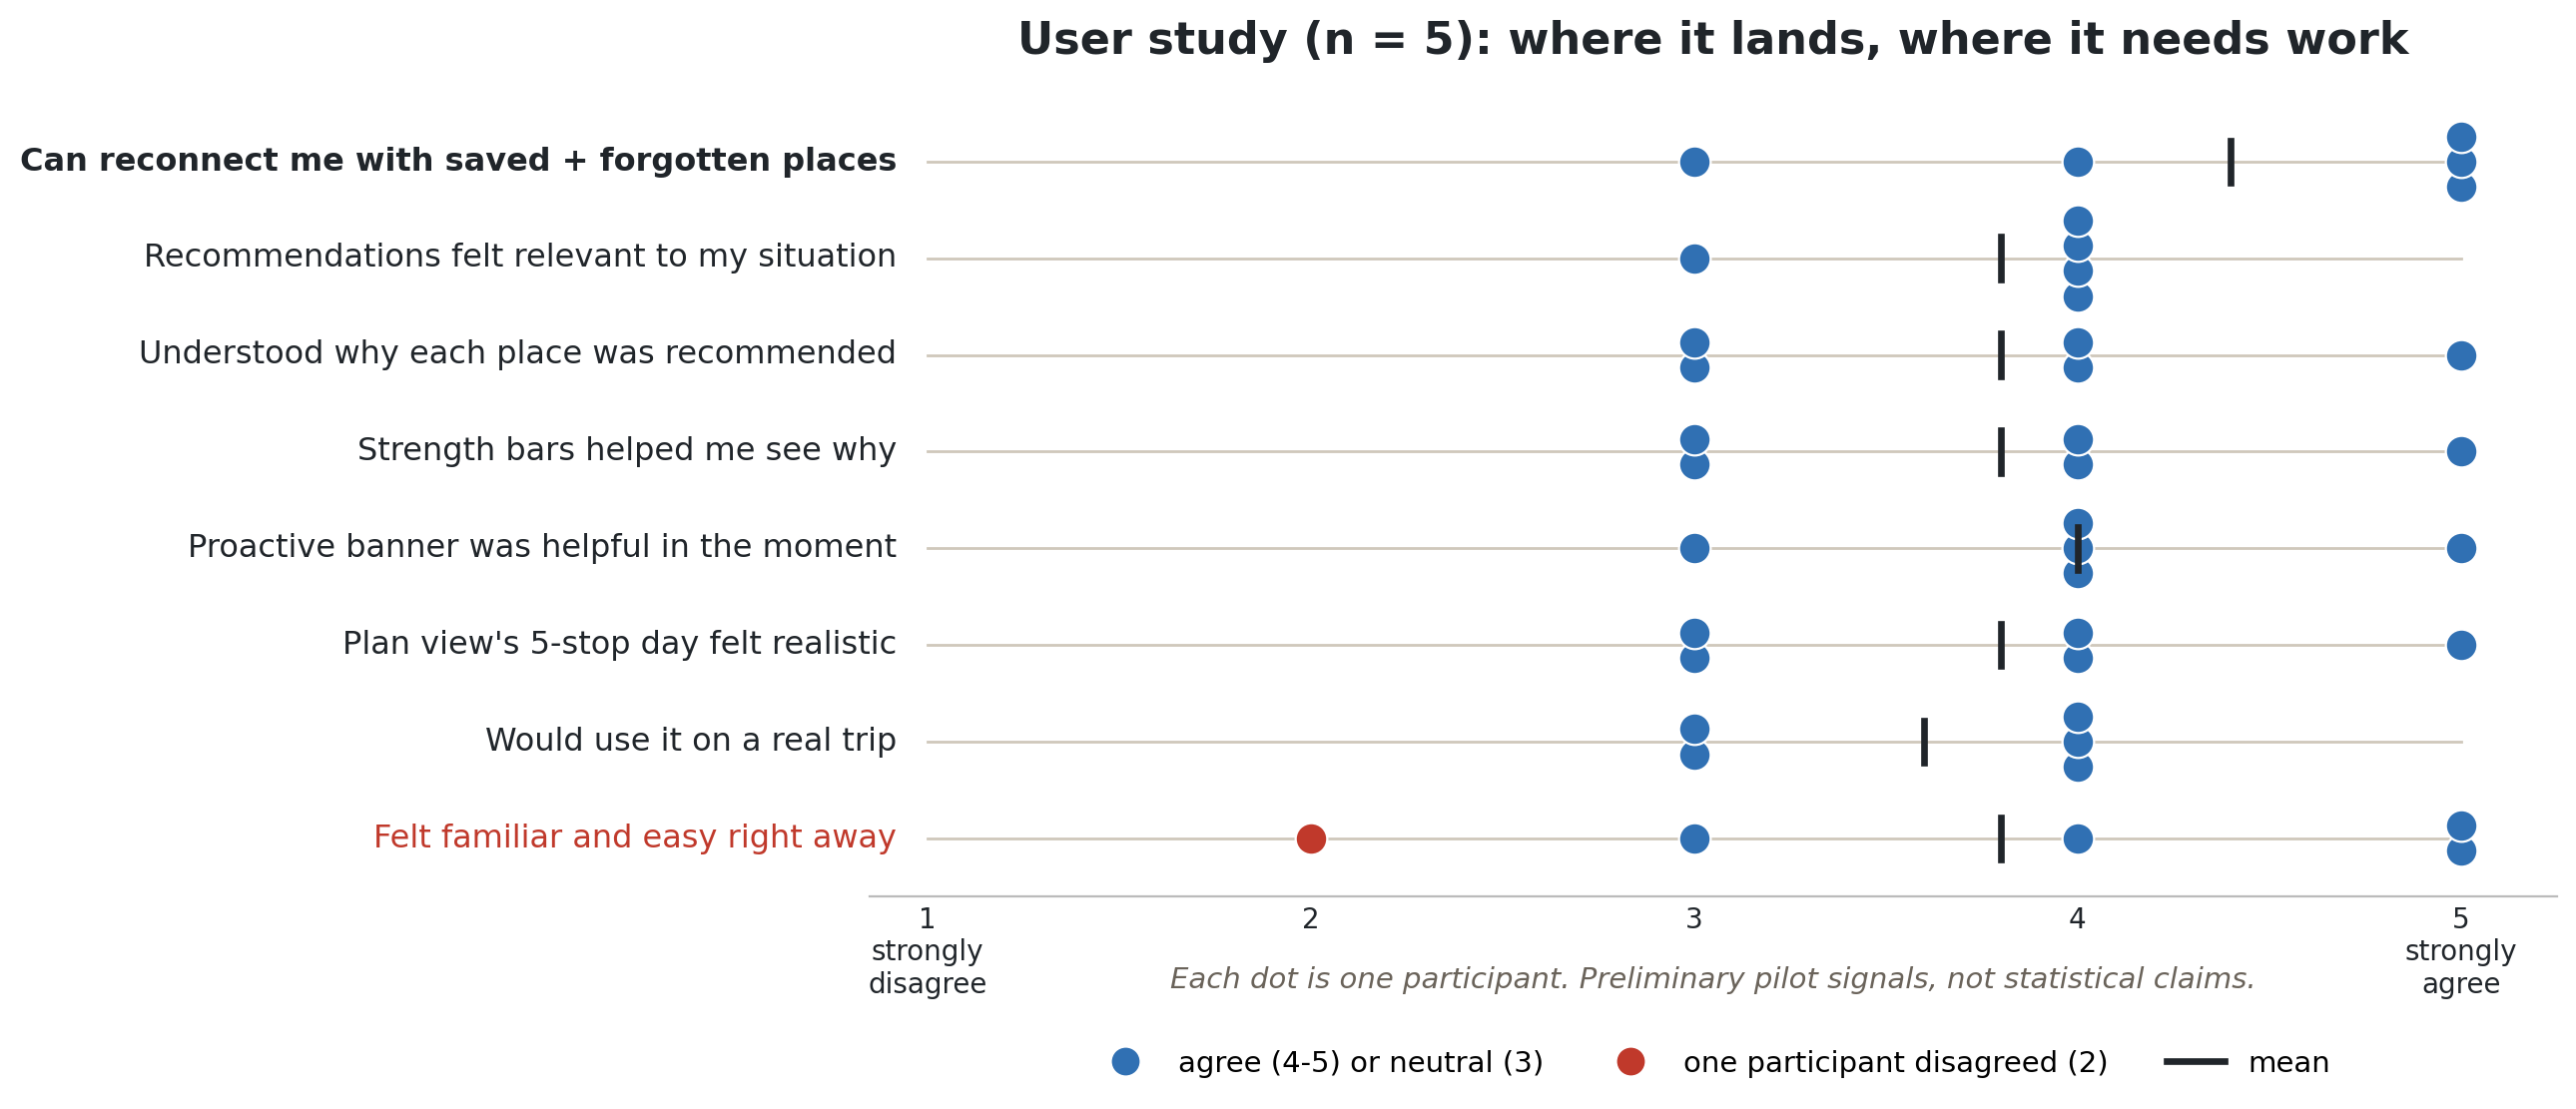
\includegraphics[width=\linewidth]{userstudy_dotplot_final.png}
  \caption{Survey responses (n=5). Each dot is one participant on a
  five-point scale. We show every response rather than aggregated
  percentages to keep the small sample visible.}
  \Description{Dot plot showing each of the five survey responses per
  statement on a five-point agreement scale.}
  \label{fig:userstudy}
\end{figure}

The statements covered the recommendations, the per-item explanations, the
proactive banner, the day plan, and overall usability;
Figure~\ref{fig:userstudy} shows every response. The strongest result
concerned re-finding itself: the statement that the app could help users
reconnect with places they had saved and forgotten clustered at agree and
strongly agree, and relevance, the explanations, and the day plan all
landed at agree or higher. The single disagreement in the survey concerned
first-run familiarity, and it points at the same issue the interviews
surfaced: the app does not explain its own purpose on first open. On the
most-useful-tab question, three of five chose ``For this moment''
(JITIR), one each chose the other two tabs, and none felt the three were
about the same. Set against the offline numbers this is informative:
``Based on history'' (CBR) records the highest offline precision, yet
users named ``For this moment'' the most useful tab. Precision measures
how well a method recovers a known target, while usefulness in the moment
depends on timing and current context, which is what JITIR is built to
serve. The gap supports the choice of JITIR as the default.

\subsubsection{Interview Findings}
Four dimensions recurred across the think-aloud sessions.

\paragraph{Explainability.}
Participants interpreted all three method labels correctly without
prompting. Several read ``Near you'' as pure distance, whereas the tab is
driven by context activation: the labels are legible at the surface, but
the algorithm behind them is not fully transparent, a target for future
explanation design. One participant independently asked for a way to
distinguish saved places that share a name, the need the personal-note
field serves, which is a small confirmation that the note-versus-name cue
of Sappelli et al.\ addresses a real problem.

\paragraph{Utility.}
Most participants found the recommendations useful; one described giving
up on places they cannot relocate, exactly the moment a recommendation
tied to the present would resurface a saved place. A more critical
response observed that re-finding neither plans the trip nor generates new
interests. This is the tension Sappelli et al.\ identify: re-finding is
distinct from discovery and lower in salience even when its value is real.
The response confirms that we targeted the right task, and that the task
is narrow by design.

\paragraph{Scalability.}
Two participants independently noted that a large saved pool calls for
organisation and routing, such as folders and time-aware planning, rather
than a three-way ranking of the entire pool. The three-method re-finding
approach suits moderate pools; large pools point toward a different
interaction paradigm. This marks the boundary of the approach without
invalidating it.

\paragraph{Trust.}
Participants trusted the per-item explanations but misread the purpose of
the system on first entry: two initially took the app for a general map or
a trip planner. Several suggested an onboarding step; we record the
request without adopting it, since consumer tourism apps are expected to
work without an instruction step. The framing of purpose therefore remains
an open design question: how to make re-finding legible at first entry
without a tutorial the category does not expect.

\subsection{Tests and CI}
\label{sec:tests}

\paragraph{Backend.}
The backend is covered by a \texttt{pytest} suite of 55 test functions
across eight modules, run against the seeded development database. The
metric implementations are pinned so they cannot drift silently:
Precision@k, Success@k, and the unique ratio are asserted against exact
hand-computed cases, and ROUGE-N and RBO against boundary and ordering
properties. Per-method tests exercise CBR, JITIR, and CIA on the seeded
pool and assert the contract every ranker must honour---results are
non-empty, correctly shaped, sorted descending, and respect
\texttt{top\_k}, with an empty pool yielding an empty result---and a
cross-method test guards against the three methods collapsing onto one
ordering. Endpoint tests cover the two data-integrity decisions of
Section~\ref{sec:backend}: reads never change the view count, the
ten-minute debounce swallows an immediate second view and admits one
after the window, and notes editing persists, clears, and ignores unknown
fields. Simulator tests assert that a seed reproduces its sessions, that
different seeds differ, and that coordinates stay inside plausible Munich
bounds, which underpins the ten-seed averaging in
Section~\ref{sec:offline}. The backend suite runs locally before results
enter the report; it is deliberately not wired into continuous
integration, since it exercises a live seeded database. The repository's
GitHub Actions workflow runs on every push and pull request and currently
covers the frontend checks: lint, the unit-test suite, and the design
check.

\paragraph{Frontend.}
The frontend suite (49 vitest tests across four modules) targets the logic
that user-visible behaviour depends on. The utilities it covers were extracted from the map page into
standalone modules precisely so they could be tested in isolation:
distance formatting, the reason-code-to-text mapper of the explanation
layer, the OSM-tag-to-category mapper behind place search, and the
method-label mapping. Two of these suites encode evaluation findings
directly. The category-mapper tests pin the three miscategorisations the
diary study surfaced (a bakery filed under shopping, a cinema and a
theatre missed as attractions) as regression cases, so a defect found in
real use cannot silently return. The label tests assert the exact
label-to-method mapping of Table~\ref{tab:method-map} against its source
of truth in \texttt{DESIGN.md}; the labels were once wired to the wrong
methods, and because the study findings are stated in terms of these
labels, an unnoticed re-wiring would invalidate the reported results, so
the mapping is enforced by a test rather than by convention. The explanation-text suite
runs against a frozen clock, keeping its time-phrase assertions
deterministic. Alongside the unit tests, the \texttt{design-check} script
of Section~\ref{sec:frontend} enforces the design-system bans statically.
A GitHub Actions workflow runs on every push and pull request: ESLint,
the vitest suite, and the design check, with the latter two gating the
build.

%% ============================================================
%% 6. CONCLUSION & FUTURE WORK   [owner: shared]
%% ============================================================
\section{Conclusion and Future Work}
\label{sec:conclusion}
% CIA row alignment resolved 2026-07-16: the checked-in 0.590 run is
% canonical (seed-time anchoring, see the caveat in Sec. 5.1); Finding 1
% finalised. Review jointly before submission.

We set out to test whether the context-aware re-finding framework of
Sappelli et al.~\cite{sappelli2017}, developed for office documents,
transfers to personal tourism information. Three findings answer that
question. First, the adaptation is faithful and the paper's central result
reproduces: across four criteria no single method dominates. CBR maximises
context precision, CIA leads rank-one action prediction and catalogue
coverage, and JITIR records the nominally strongest top-ten action score,
so the methods are complementary rather than ranked.
Second, the ordering that holds in the offline simulator also holds on
real, accumulated data: over a week of the authors' own use the three tabs
visibly separated, and the context signals responded to time and weather. Third, re-finding is a real but
\emph{low-salience} need. Participants trusted and valued the per-item
recommendations and named the moment-aware JITIR tab the most useful, a
preference that independently supports its choice as the default; yet
several initially misread the app as a map or a planner. The evaluation
therefore locates the value at the item level and the open problem at the
system level, in how the application conveys its purpose on first entry.

Future work follows the seams the evaluation exposed. On the modelling side,
the offline evaluation should move from a simulator to \emph{real}
interaction logs, and the CIA connection weights, currently the paper's
fixed Table-3 heuristics, could be learned from those logs. The time-of-day
signal should become timezone-aware and per-venue rather than per-category.
The data model stores an event time on saved items, and CIA already
consumes it as a coarse time-of-day context node; but nothing yet
\emph{triggers} on the approaching time itself, and the save flow does not
let users set one. A \emph{time-anchored} proactive trigger (surfacing a
ticket or reservation as its time approaches) would be a stronger
re-finding signal than the current category-and-proximity cues. On the product side, the study
points to first-run framing of the re-finding concept, better place-search
coverage and disambiguation, arbitrary-origin transit routing, and an
organisation-and-routing mode for the large saved pools that participants
anticipated. Finally, a larger user study would convert the present
directional evidence into measurement.

%% ============================================================
%% ETHICS & PRIVACY  (ACM template asks for this; keep ~3 sentences)
%% ============================================================
\section*{Ethics and Privacy Statement}
\addcontentsline{toc}{section}{Ethics and Privacy Statement}
% DRAFT (shared section) --- review jointly before submission.
The user study was small, voluntary, and anonymous; participants were
informed of the tasks and consented to session recording. The deployed
prototype is a single shared demo pool without user accounts: the pool is
initialised from a curated seed set that users extend with their own
saves, and the only identifier attached to interactions is a hard-coded
anonymous client id. Feedback events store a coarse context snapshot
(coordinates and time of the judgement) used solely for per-method
evaluation; no names, contact details, or persistent personal identifiers
are collected, and nothing is shared with third parties. The serving path
makes no live model calls; the only external call at runtime is the
client's weather fetch to the keyless Open-Meteo API, pinned to Munich
coordinates. Diary-study entries were recorded by the authors about their
own use of the application.

%% ============================================================
%% GenAI DISCLOSURE  (REQUIRED by the course; does NOT count to page limit)
%% ============================================================
\section*{GenAI Disclosure}
\addcontentsline{toc}{section}{GenAI Disclosure}
% DRAFT --- edit to reflect your actual usage honestly before submission.
The design direction, research framing, method choices, and all evaluation
decisions in this project are the authors' own. Generative AI tools
(Claude Code) were used as a coding and drafting assistant under
author-defined constraints: for code refactoring and feature implementation
against specifications the authors set, and for drafting and structuring
prose from author-provided decisions, notes, and results. All technical
claims, algorithm descriptions, and reported numbers were verified by the
authors against the implementation and the experimental output. The authors
take full responsibility for the content of this report.

%% ============================================================
%% BIBLIOGRAPHY
%% Put refs in references.bib ; cite with \cite{key}. Key one: Sappelli 2017.
%% ============================================================
\phantomsection
\addcontentsline{toc}{section}{References}
\bibliographystyle{ACM-Reference-Format}
\bibliography{references}

%% ============================================================
%% APPENDIX (max 2 pages) - optional extra figures/tables
%% ============================================================
\appendix
\section{Additional Material}
\label{sec:appendix}
Figure~\ref{fig:overview} collects the per-metric comparisons for all four
methods across the six offline metrics, complementing the analysis of
Section~\ref{sec:offline}.

\begin{figure}[h]
  \centering
  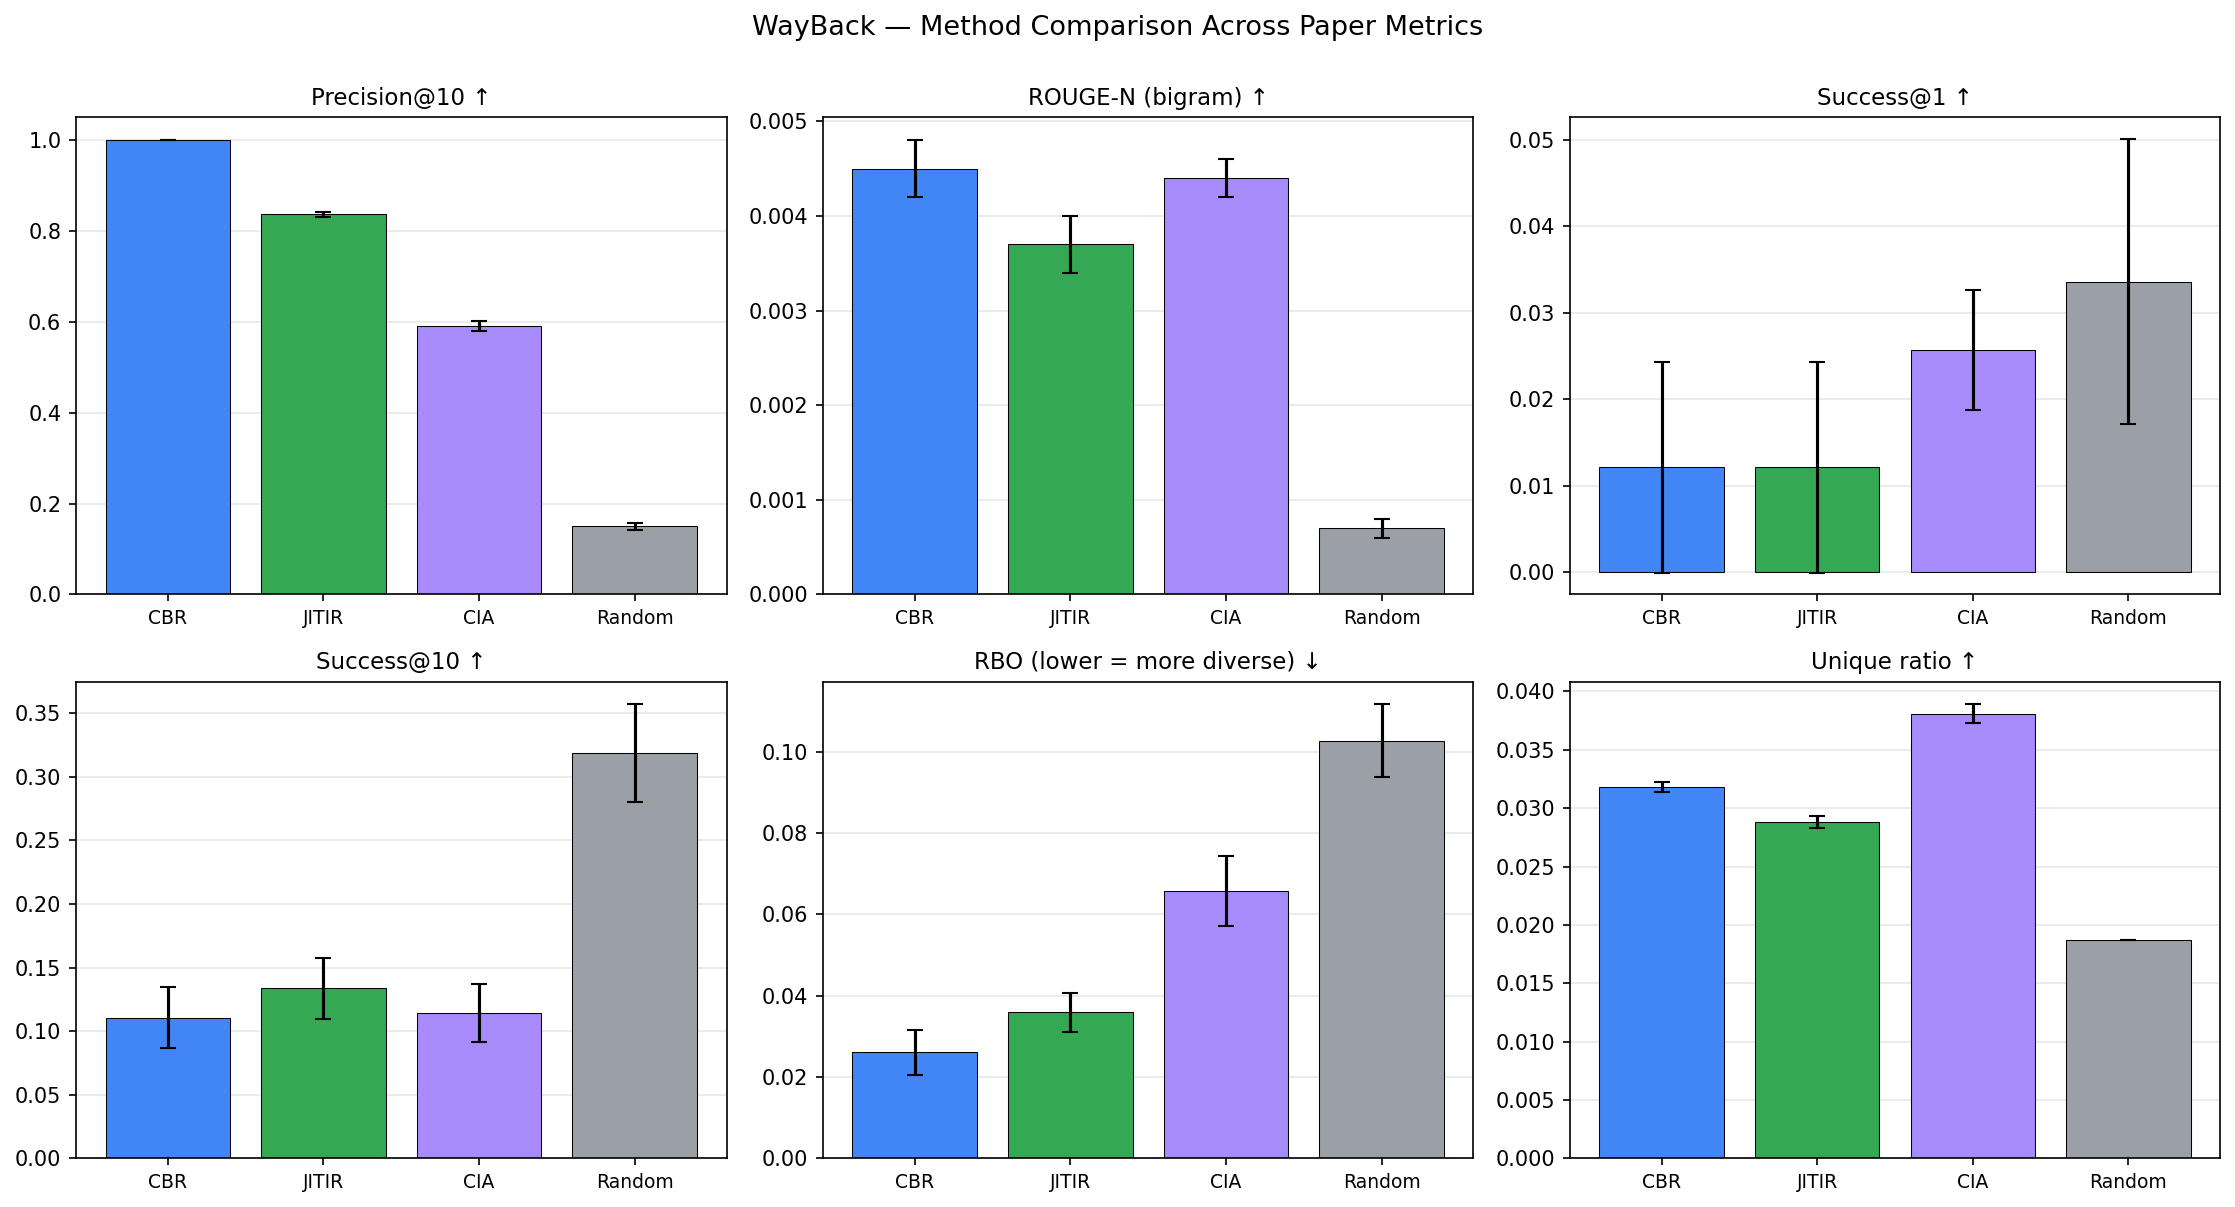
\includegraphics[width=\linewidth]{plot_overview.png}
  \caption{Offline metric comparison across all four methods (mean over ten
  seeds). Higher is better for every panel except RBO, where lower means
  more responsive to context.}
  \Description{Six-panel chart comparing CBR, JITIR, CIA, and random across
  the six offline metrics.}
  \label{fig:overview}
\end{figure}

%% ============================================================
%% CONTRIBUTIONS TABLE  (REQUIRED; does NOT count to page limit)
%% Full names as on TUM transcripts, GitHub handles, contributions.
%% ============================================================
\section{Author Contributions}
\begin{table}[h]
  \caption{Author contributions}
  \begin{tabular}{llp{7cm}}
    \toprule
    Full name & GitHub handle & Contribution \\
    \midrule
    Haichen Duan & Haichennn & Frontend, UI/UX, design system, frontend CI (lint, unit tests, design-check on GitHub Actions), user study, diary study and visualization\\
    Swayamsidh Mohanty & dhalakau & Backend, recommender method implementations, backend tests, evaluation pipeline, deployment\\
    \bottomrule
  \end{tabular}
\end{table}

\end{document}
